\begin{figure*}[htbp]
\centering
\begin{tikzpicture}
\pgfplotsset{compat=1.16}
\node at (0,0) {\begin{tikzpicture}\begin{axis}[ybar,width=0.49\textwidth,height=5.2cm,bar width=2.2pt,symbolic x coords={afr,amh,ewe,hau,ibo,kin,lin,lug,nso,orm,sna,som,swh,tir,tsn,twi,wol,xho,yor,zul},xtick=data,x tick label style={rotate=90,font=\tiny},ylabel={chrF++ minus greedy},title={SFT baseline},title style={font=\small},ymajorgrids,tick label style={font=\scriptsize},label style={font=\scriptsize},enlarge x limits=0.04,legend style={font=\tiny,at={(1.1,-0.62)},anchor=north,legend columns=3}]
\addplot[fill=blue!60,draw=none] coordinates {(afr,-1.147) (amh,6.592) (ewe,-0.469) (hau,2.233) (ibo,-1.049) (kin,7.625) (lin,9.408) (lug,7.115) (nso,12.180) (orm,9.419) (sna,3.205) (som,0.127) (swh,0.180) (tir,6.490) (tsn,5.400) (twi,3.351) (wol,1.607) (xho,-0.660) (yor,3.423) (zul,-0.824)};
\addplot[fill=orange!80,draw=none] coordinates {(afr,0.919) (amh,1.062) (ewe,-5.376) (hau,-1.401) (ibo,0.266) (kin,0.913) (lin,0.787) (lug,-4.266) (nso,5.900) (orm,-1.372) (sna,4.079) (som,0.914) (swh,3.975) (tir,1.865) (tsn,3.393) (twi,-0.800) (wol,0.795) (xho,2.024) (yor,3.242) (zul,2.029)};
\addplot[fill=green!50!black,draw=none] coordinates {(afr,0.657) (amh,7.902) (ewe,3.868) (hau,3.874) (ibo,1.837) (kin,8.563) (lin,12.022) (lug,10.686) (nso,14.336) (orm,14.419) (sna,4.847) (som,3.262) (swh,3.807) (tir,6.722) (tsn,6.429) (twi,5.189) (wol,3.625) (xho,1.911) (yor,3.817) (zul,1.424)};
\end{axis}\end{tikzpicture}};
\node at (8.4,0) {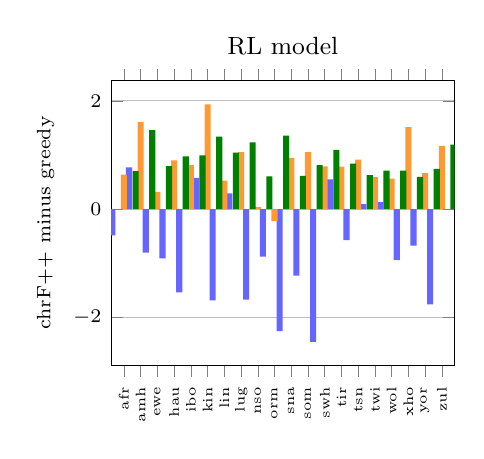
\begin{tikzpicture}\begin{axis}[ybar,width=0.49\textwidth,height=5.2cm,bar width=2.2pt,symbolic x coords={afr,amh,ewe,hau,ibo,kin,lin,lug,nso,orm,sna,som,swh,tir,tsn,twi,wol,xho,yor,zul},xtick=data,x tick label style={rotate=90,font=\tiny},ylabel={chrF++ minus greedy},title={RL model},title style={font=\small},ymajorgrids,tick label style={font=\scriptsize},label style={font=\scriptsize},enlarge x limits=0.04,legend style={font=\tiny,at={(1.1,-0.62)},anchor=north,legend columns=3}]
\addplot[fill=blue!60,draw=none] coordinates {(afr,-0.487) (amh,0.773) (ewe,-0.803) (hau,-0.913) (ibo,-1.539) (kin,0.579) (lin,-1.689) (lug,0.292) (nso,-1.671) (orm,-0.880) (sna,-2.255) (som,-1.228) (swh,-2.452) (tir,0.550) (tsn,-0.575) (twi,0.093) (wol,0.131) (xho,-0.941) (yor,-0.674) (zul,-1.759)};
\addplot[fill=orange!80,draw=none] coordinates {(afr,0.637) (amh,1.614) (ewe,0.319) (hau,0.899) (ibo,0.815) (kin,1.937) (lin,0.525) (lug,1.054) (nso,0.041) (orm,-0.220) (sna,0.945) (som,1.055) (swh,0.789) (tir,0.787) (tsn,0.915) (twi,0.595) (wol,0.565) (xho,1.514) (yor,0.664) (zul,1.167)};
\addplot[fill=green!50!black,draw=none] coordinates {(afr,0.701) (amh,1.459) (ewe,0.795) (hau,0.977) (ibo,0.991) (kin,1.342) (lin,1.044) (lug,1.235) (nso,0.605) (orm,1.359) (sna,0.614) (som,0.811) (swh,1.095) (tir,0.842) (tsn,0.630) (twi,0.710) (wol,0.710) (xho,0.595) (yor,0.744) (zul,1.193)};
\end{axis}\end{tikzpicture}};
\end{tikzpicture}
\caption{E-02 per language: chrF++ gain of beam search (4 beams, primary and HF rule) and MBR (16 samples) over greedy decoding, for the SFT baseline (left) and the RL model (right); 20 FLORES+ languages, 200 sentences each. Bars: blue = beam-4, orange = beam-4 (HF rule), green = MBR-16; bars above zero help. The baseline gains a lot in many languages and the RL model little; intervals per language are in Tables~\ref{tab:dec-d-sft-pp} and~\ref{tab:dec-d-rl-pp}.}\label{fig:dec-per-language}
\end{figure*}
